% =====================================================================
% SESAR Innovation Days 2026 -- submission draft
%
% THIS IS A DRAFTING SCAFFOLD, NOT THE OFFICIAL SID TEMPLATE.
% The official page states: "Templates in word and latex format are
% available for download on the submission page and shall be used to
% create the submission." Before submitting, transplant this text into
% the official template from EasyChair and re-check the page count there.
% See COMPLIANCE.md for what was verified and what was not.
%
% Review is NOT blind for this edition (organisers confirmed 2026-08-06,
% see COMPLIANCE.md): the author block is visible via \blindfalse below.
% An earlier version of this header wrongly said triple-blind.
% =====================================================================
\documentclass[conference,10pt,a4paper,IEEEoverridecommandlockouts]{IEEEtran}

\usepackage[utf8]{inputenc}
\usepackage[T1]{fontenc}
\usepackage{booktabs}
\usepackage{graphicx}
\usepackage{amsmath}
\usepackage{url}
\usepackage[hidelinks]{hyperref}
\usepackage{balance}
\graphicspath{{figures/}}
% modest float-separation tightening; IEEEtran defaults leave generous gaps
\setlength{\textfloatsep}{7pt plus 2pt minus 3pt}
\setlength{\dbltextfloatsep}{7pt plus 2pt minus 3pt}


% Typesetting: no single line of a paragraph may be stranded at the top or
% the bottom of a page or column, and no word may be hyphenated across a
% page break. These are the standard penalties; they cost a little vertical
% justification and buy pages that read continuously.
\usepackage{stfloats}
\clubpenalty=10000
\widowpenalty=10000
\displaywidowpenalty=10000
\brokenpenalty=10000
% Two columns cannot both be filled to the last line once those
% penalties hold, so the bottoms are allowed to differ rather than
% stretched: a stretched column shows as visible gaps between the
% paragraphs, which is worse than a short column.
\raggedbottom

\begin{document}

\title{Which Reroute Will an Airline Accept?\\Learning Route Preferences from Revisions}

% SID 2026 review is NOT anonymous (confirmed with the organisers), so
% \blindfalse is the correct setting. \blindtrue is kept only in case the
% policy changes.
\newif\ifblind
\blindfalse

\ifblind
  \author{\IEEEauthorblockN{Anonymous submission}
  \IEEEauthorblockA{Author details withheld}}
\else
  \author{%
  \IEEEauthorblockN{Ramon Dalmau\textsuperscript{1}, David
  Perez\textsuperscript{2}, Franck Ballerini\textsuperscript{1}, Seddik
  Belkoura\textsuperscript{2},\\ Vincent Taverniers\textsuperscript{2},
  Gratiel Marius Marin\textsuperscript{2}, Robin
  Deransy\textsuperscript{1}, Benjamin Cramet\textsuperscript{3} and Grigori
  Gustin\textsuperscript{3}}
  \IEEEauthorblockA{EUROCONTROL\\
  \textsuperscript{1}Innovation Hub, Br\'etigny-sur-Orge, France \quad
  \textsuperscript{2}Maastricht UAC, the Netherlands \quad
  \textsuperscript{3}Headquarters, Brussels, Belgium}}
\fi

\maketitle

\begin{abstract}
When an airline revises the route in a flight plan, the revision records
a choice it actually made: the route it dropped and the route it filed
instead. Each such pair
carries the key performance indicators of both routes (planned fuel,
flight time, en-route charges and attributed delay) together with the
waypoint sequence each route follows. This paper treats 1.48 million such
pairs from eighteen months of European traffic as revealed preferences and
trains a pairwise ranking model to predict which of two candidate routes
an airline would choose. On a held-out test set the model never saw during training, it identifies
the chosen route 68.1\,\% of the time, against 55.0\,\% for the
strongest single-indicator rule. On the fifth of pairs where the model is
most confident, it reaches 94.9\,\%. Because its confidence is
calibrated, the model can support a proposal channel that offers
fuel-saving routes only where they are likely to be accepted, at a
precision chosen in advance. A simulation of such a channel against the
airlines' own later filings reaches 79.2\,\% precision and surfaces
20.1\,kilotonnes of planned-fuel savings in a single quarter.
% Cut for space and for the author's 2026-09-07 instruction that the
% abstract be an overview of the paper rather than a summary of its
% results: the detail below is reported in Sections IV-B and V.
% (94.9\,\% on the top fifth restored to the abstract on 2026-09-08.)
% ... Aimed at 80\,\% and then measured on a held-out
% quarter, such a channel reached 79.2\,\% and surfaced 56\,162
% proposals carrying a planned-fuel saving of 20.1 kilotonnes over the
% quarter that the airlines' own later filings confirm, or 222 to 254
% kilotonnes of CO$_2$ a year on two annualisation bases.
% ... preferring the route with less planned fuel scores 45.0\,\% ...
% thirteen points below the model ... apart from 1\,093 held-out pairs in
% which a flight kept its route ...
\end{abstract}

\begin{IEEEkeywords}
air traffic flow management, airline preferences, learning to rank,
fuel efficiency
\end{IEEEkeywords}

% =====================================================================
\section{Introduction}
\label{sec:intro}

On a spring morning in 2026, an Airbus A320 was filed from Amsterdam to
Barcelona on a route carrying 102 minutes of attributed air traffic flow
management (ATFM) delay, and the operator subsequently re-filed. The new
route shed that delay completely, and it cost the airline on each of the
three counts it pays for directly: 39 minutes of flight time,
1\,397\,kg of extra planned fuel, and 466 euros more in en-route charges.
Both routes are held in the network's records and so, implicitly, is the
operator's judgement that the delay would have cost it more than the
detour did.
% CORRECTED 2026-09-07: the paragraph listed what the detour cost but
% omitted en-route charges, the third of the three costs the paper uses
% throughout. Verified for this pair in
% data/ich_dataset/ich_dataset_2026-05.parquet, pair_id 1421263:
% kpiRouteChargeIndicator 1274 -> 1740 EUR (units per run_01_eda.py:41).


That judgement is the quantity this paper models. A flight plan is not
filed once and left alone: an airline may revise it at any time until the
aircraft leaves. An operator may reroute to avoid ATFM delay and prevent
it from propagating to subsequent legs, or it may reroute because updated
weather reveals a more fuel-efficient alternative. The archive records
what changed rather than why, and every revision leaves the same trace:
the route replaced and the route that replaced it.


% Cut for space 2026-09-08: PRC extra-distance paragraph
% (\cite{prc2026}) replaced by the revealed-preference motivation below,
% at the author's request. Original text:
% "The scale of what is at stake is published every year. The Performance
% Review Commission reports how much further European traffic flies than a
% direct reference between the points at which it enters and leaves the
% airspace. Not all of that distance is avoidable: airspace that cannot
% take all the traffic that wants it has to be protected, and a flight
% routed around it flies further, so part of the figure is what respecting
% a limited capacity costs. What this paper takes up is whether any of the
% rest is a cheaper route that the operator would have been willing to fly
% and did not file. That such routes exist is assumed here rather than
% shown."
The network records over a million such revisions a year across European
airspace. A regulation may occasionally leave no viable alternative, but
most revisions record a genuine preference: the operator had two routes
available and filed the one it preferred. If those preferences could be
predicted, a route proposal that saves fuel need not be offered blind; it
could be aimed at the flights whose operators would file it.

Candidate routes are not hard to come by. What is hidden is how each
operator weighs them: the balance between fuel, flight time, en-route
charges and delay differs by airline and by day, and no airline publishes
it. The terms of that trade-off, however, are recorded for every route in
the network's operational data, and so is the outcome: the route the
airline actually filed. A preference model fitted to enough such
observations can learn the underlying weighting without access to any
operator's cost function.
% Cut for space (the same point is made where deployment is discussed):
% needless to say, proposing routes that airlines reject is worse than
% proposing nothing at all, because a channel that is ignored is a channel
% that is eventually switched off.

The contribution of this paper is threefold. First, it shows that
airline route acceptance is learnable at network scale from revision
events alone, and that the confidence of the resulting model
is calibrated well enough to support a chosen operating point rather than a
single accuracy figure. Secondly, it argues that the label construction is
itself a design decision worth defending: a revision pair records a
preference the airline actually expressed. The usual alternative ranks the
filed route above candidates produced by a route generator, a comparison
the operator may never have been shown. Thirdly, it reports
what the model has learned rather than only how well it scores,
namely that route structure outweighs any single cost indicator, together
with the caveats that such an attribution demands.

The remainder of this manuscript is organised as follows.
Section~\ref{sec:background} explains why a pair of routes drawn from a
revision constitutes a preference observation and what a model of such
observations is for, and Section~\ref{sec:related}
positions the work within the literature on rerouting and route choice.
Section~\ref{sec:method} describes the archive, the split protocol and the
model, while Section~\ref{sec:results} reports the results. Finally,
Section~\ref{sec:conclusions} concludes and outlines future work.

% =====================================================================
\section{Background} \label{sec:background}

This section explains how a flight-plan revision becomes a labelled
preference pair, why that label is preferred to one built from generated
candidates, and what the model is for.

\subsection{Flight-plan revisions as preference data}

In the European network a flight plan is filed before departure and may be
revised until the flight leaves. Every filing is a message, and so is every later change. The network
keeps them all, so what it holds for a flight is the whole sequence of
messages sent for it. A route change
is accordingly a pair of consecutive messages rather than a record of its
own: the message that changed the route, and the one it
replaced. 

\begin{figure*}[t]
\centering
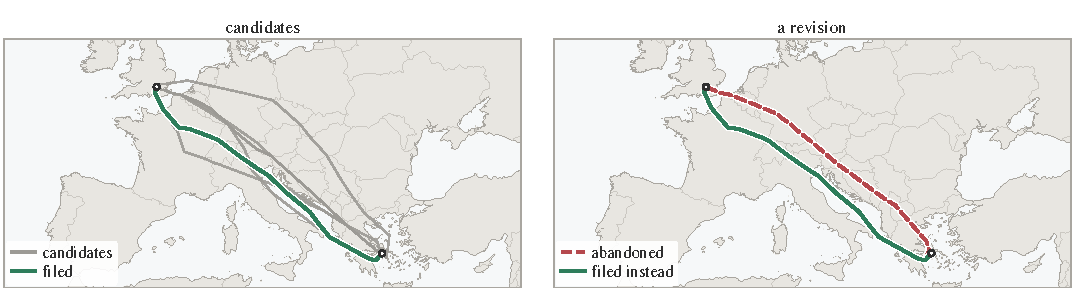
\includegraphics[width=\textwidth]{pair_idea.pdf}
\caption{Two ways to build a training pair, on one city pair. Left: the
filed route (solid green) is ranked above candidates a route generator
would supply (grey); the grey tracks drawn here are real routes flown on
the same city pair,
standing in for generated ones. Right: a revision supplies two routes that
the same operator filed for the same flight hours apart, one of which it
abandoned. Only the right-hand pair records a preference the airline
actually expressed.}
\label{fig:pairidea}
\end{figure*}

The two together describe a decision, because the operator had
committed to the earlier route and then filed the later one for the same
flight, which makes the later route the one it chose and
the earlier one the route it abandoned.

The sharpest of those decisions are made under flow management. When the
traffic expected in a volume of airspace exceeds what can
safely be handled there, whether because of demand, staffing, weather or
equipment, a \emph{regulation} is placed on it and the flights crossing it are given calculated take-off times at
the rate it can absorb; the difference between a flight's calculated
and requested take-off times is its ATFM delay.

An
operator facing an ATFM delay has a choice that is genuinely
economic: accept it, or file a route that avoids the constrained
volume at the cost of distance, fuel and en-route charges, and neither
answer is universally correct. For instance, a flight with a tight
aircraft rotation may find forty minutes of delay far more expensive than a
tonne of fuel, whereas the same delay on the last leg of the day may well be
cheaper than the detour. This is why the decision is worth learning rather
than deriving: the costs that determine it are operator-specific and
flight-specific, and the network does not observe them, though the
outcomes of those trades are recorded. Published European reference
values~\cite{cook2015} give the order of magnitude of the cost of delay
and are widely used for analysis, but they are not the cost function
any particular operator applies.

Most revisions, though, are not a response to flow management at all.
Seven pairs in ten in this archive carry no regulation on either route
(Table~\ref{tab:composition}), and within those the two routes differ by
a median of one kilogramme of planned fuel. 

% Cut for space (Table~\ref{tab:composition} now reports this directly):
% the archive reflects this trade, in that slightly under a third of the
% revision pairs carry a regulation on either route and the newly filed
% route is more often longer, slower and more fuel-intensive than the one
% it replaced.

The same events also settle how the training labels are built, because
which of two routes an operator prefers cannot be asked at network
scale but it can be observed, and the labels used herein follow the
logic of revealed preference (i.e., inferring what an actor values
from the choice it made when a concrete alternative was
available)~\cite{samuelson1938}.

The alternative label construction, adopted by the authors' own earlier work,
ranks the filed plan above candidates supplied by a route
generator~\cite{dalmau2024}. Its weakness is not that such routes are
unrealistic. It is that nobody knows whether any of them ever reached the
dispatcher who planned the flight. The label asserts that the operator
preferred the filed route to the generated one, whereas all the record
shows is that the operator filed one route, so the comparison the label
claims may never have taken place at all.

A revision pair claims nothing that did not happen, and
Fig.~\ref{fig:pairidea} draws the two constructions side by side on one
city pair. Both routes of a revision reached the dispatcher's screen,
since the operator filed each of them in turn, for the same flight, on the
same day. The route labelled less preferred is therefore not a plausible
alternative constructed after the fact but one the operator had committed
to and then abandoned, which makes the training signal a comparison that
demonstrably took place.



Ranking a filed plan above generated candidates may require only that the
model
recognise which route looks like a filed plan, which is a different and
much easier skill than knowing which route an operator would prefer. For instance, a generated candidate
may join published segments in a way no dispatcher would ever file, so
that telling it from a filed plan can be done on the shape of the route
alone, without knowing anything about the operator that would fly it.

% Cut for space 2026-09-08: "No dataset offers both label sources for
% the same flights, so the comparison between the two constructions is
% conceptual rather than measured. The prediction task is itself narrow:
% given two specific routes, the model says which the airline would
% prefer. That is the question a proposal channel needs answered."
% Removed because the label argument is made in the preceding paragraphs,
% the pairwise task is established in the abstract, and the channel's
% needs are covered in Section II-B.

% Cut for space (Section IV-A states this trap in full, with the same
% forward reference to Section V-B):
% The price to be paid is that revisions are not a random sample of
% flights, but rather flights that changed, which introduces a bias of
% its own. Rather than assuming that bias away, Section~\ref{sec:changebias}
% measures it.

\subsection{Two operational use cases}
\label{sec:usecases}

The first use case is a proposal channel:
propose to an airline a route that is more fuel-efficient than the
one it filed and that the model deems likely to be accepted, on the
grounds that the operator may not have seen or evaluated that alternative
in time. Calibrated confidence is what makes the channel viable: because the
model's score estimates the true probability of acceptance, choosing a
threshold directly sets the precision of the proposals. A stricter threshold
means fewer proposals but a higher fraction that the airline would
accept, so the channel can be tuned to a point where it stays credible
rather than being ignored. 

\begin{figure*}[!h]
\centering
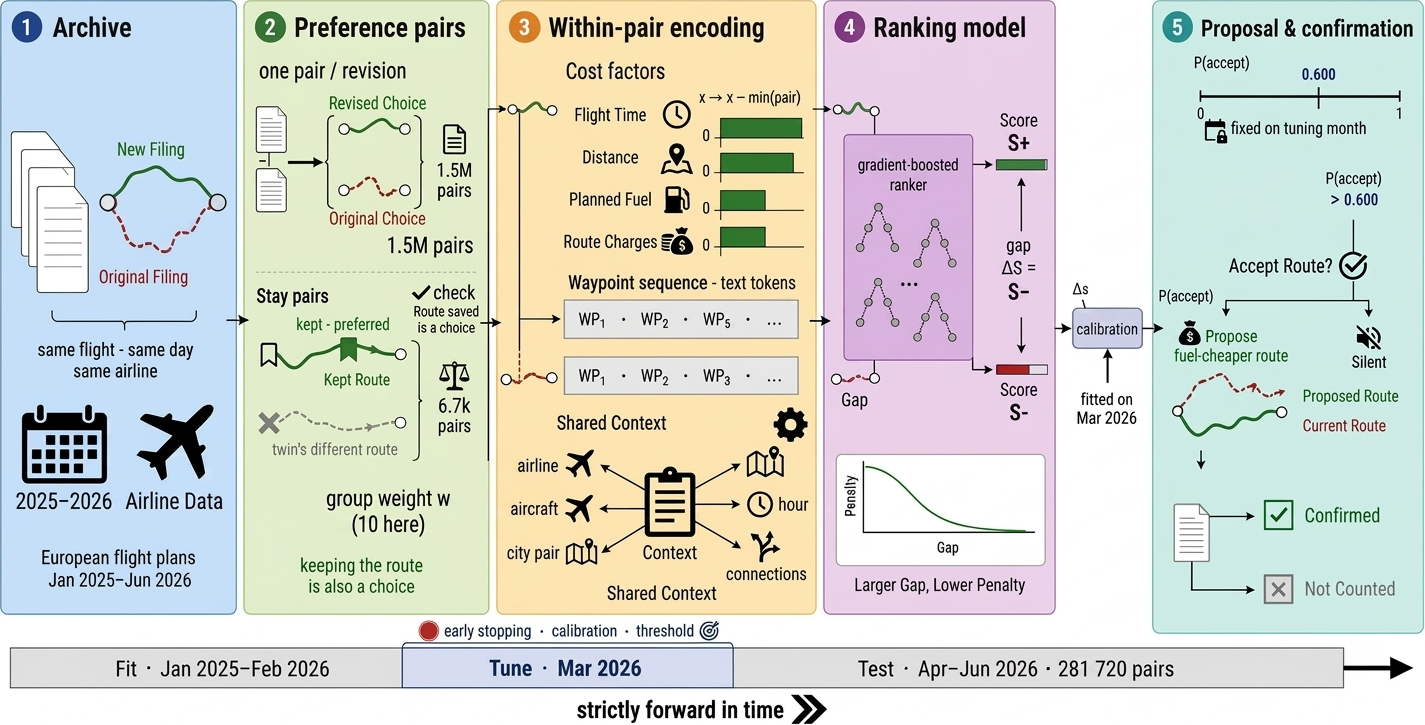
\includegraphics[width=\textwidth]{fig_pipeline.png}
\caption{How a filing archive becomes a proposal, above the fit, tune
and test periods. The pair box shows both constructions: a revision,
which is one flight and two routes, and a stay pair, which is two
flights. The inset in the fourth stage is the training objective, whose
penalty falls as the gap between the two scores widens and never reaches
zero; the calibrated probability against its threshold is the only
condition on a proposal. The bars of the third stage are one illustrative
pair, in which the chosen route is the costlier on each indicator, the
commoner direction on this archive rather than the invariable one.}
\label{fig:method}
\end{figure*}

The second use case is overload release: when a traffic volume is
overloaded and flights may be rerouted out of it, someone must decide
which flights to approach first. At present, that ranking has no
systematic basis in acceptance likelihood. Ranking flights by whether an
acceptable and more fuel-efficient alternative exists would let the network manager relieve the overload while approaching
fewer operators and asking less of each.

Neither use case is tested end to end here: this paper demonstrates the
preference model on which both depend, and simulates the first against
the airlines' later filings.
% Cut for space: both use cases return data to the model that drives them,
% since every proposal answered and every release accepted is a new labelled
% observation, so the preference model improves with use; responses would,
% however, be a biased sample of the flights the channel itself selected,
% which is why the shadow-mode trial proposed in the conclusions comes
% first.

% =====================================================================
\section{Related work} \label{sec:related}

Work on rerouting in ATFM has largely approached the
problem from the network side. Over two decades ago, the authors of~\cite{bertsimas2000} formulated
rerouting as a dynamic network flow problem, and the authors
of~\cite{mukherjee2009} subsequently added a stochastic model that reroutes
flights as capacity evolves. Both optimise an objective defined by the
network and assume, in effect, that the resulting assignment is executed, so
that the willingness of the airline to fly it is not modelled.

More recently, route choice in Europe was studied as a trade between
fuel and en-route charges~\cite{delgado2015}, which establishes that the
choice is economic and therefore learnable, but uses no label in which the
operator rejected an alternative it had itself filed. The closest work to the present one is that of the authors
of~\cite{murca2018}, who incorporate airline preferences into collaborative
rerouting decisions and show that accounting for them changes which reroutes
are selected. Those preferences, however, are inputs to an optimisation,
whereas this paper learns the preference function itself, at network scale,
from what airlines did rather than from what they stated.
% Cut for space (both are in the journal extension): Airline input already
% reaches flow management in two other places, neither of them route
% choice: the collaboration whose value~\cite{castelli2012} establishes,
% which motivates the channel simulated herein but says nothing about
% which proposals would be taken up, and the user-driven prioritisation
% process (UDPP)~\cite{pilon2021}, which orders delay among an operator's
% own flights.

The direct predecessor of this work applies learning to rank to flight routes
for a different purpose: predicting the flight plans that have not yet been
filed, so that traffic demand can be estimated earlier than the filing horizon
allows~\cite{dalmau2024}. 

That work established the framing adopted herein, namely a gradient-boosted
ranker that scores routes by their indicators in context, and it reported
the very difficulty that motivates the present paper. Its training pairs take the filed plan as preferred and a set of generated
proposals as less preferred, which is the construction that
Section~\ref{sec:background} argues against.



% =====================================================================
\section{Methodology} \label{sec:method}

Figure~\ref{fig:method} shows the procedure end to end; the two
subsections that follow cover the data and the model.

\subsection{Data and pair construction}

Eighteen consecutive months of European network data, from January 2025 to
June 2026, are used. After retaining only those revisions that change the
horizontal route, and only those pairs with complete key performance
indicators, the archive contains 1.48 million labelled pairs.



What those decisions look like matters before any model touches them, and
Table~\ref{tab:composition} breaks the archive down by the regulation
context in which each revision was made.
% Cut for space 2026-09-07 (Section II-A now states the same two figures,
% which it must, because a reader who does not know that most revisions
% are unregulated misreads the whole of Section II):
% Seven revisions in ten are made with no regulation on either route,
% and the median fuel difference across them is one kilogramme.
The unregulated majority differs by a median of one kilogramme of planned
fuel, and the pairs that cost fuel are elsewhere: the revisions that
escape a delay outright, or reduce one, together account for 18.4\,\% of
the archive.

A revision that escapes a delay moves to a route burning a
median 101\,kg more than the one it replaced, and that route burns less fuel in only 28.1\,\% of cases; a revision
that merely reduces the delay costs a median 65\,kg and is more
fuel-efficient in 31.6\,\%. 

\begin{table}[t]
\caption{The revision archive by decision context, over all eighteen months.
A route counts as regulated when the flight, while filed on that route,
had a regulation attributed to it, which leaves the delay itself free to
be zero. Unregulated pairs carry no
regulation on either route, escapes carry one on the abandoned route only,
the next two carry one on both, and the last only on the newly filed route.
The fuel difference is between the two routes of a pair.}
\label{tab:composition}
\centering\footnotesize
\setlength{\tabcolsep}{3pt}
\begin{tabular}{lrrrr}
\toprule
context & pairs & share & median $\Delta$fuel & new route \\
        &       & [\%]  & (new $-$ old) [kg]  & burns less [\%] \\
\midrule
unregulated          & 1\,047\,228 & 70.6 & 1    & 46.2 \\
escaped delay        & 117\,594    & 7.9  & 101  & 28.1 \\
reduced delay        & 155\,326    & 10.5 & 65   & 31.6 \\
kept or raised delay & 141\,648    & 9.6  & 0    & 47.4 \\
took on delay        & 21\,337     & 1.4  & $-5$ & 51.8 \\
\bottomrule
\end{tabular}
\end{table}

Each route is described by twenty-three features, summarised in
Table~\ref{tab:features}. The two routes of a pair are separated in time as
well as in geography, however, and that must be addressed before
anything is learned. The replacement is by
construction the later message, so any feature that drifts with time
identifies the answer without saying anything about the quality of the
route. The time remaining to departure is the clearest case: it is
necessarily smaller for the route that replaced the other, so a model given
it in raw form could answer ``the one filed later'', be right on essentially
every pair, and know nothing whatever about routes. This is leakage rather
than learning, and it would be invisible in the accuracy figure.

To ensure a
fair comparison between the two routes, every flight-level attribute was
therefore harmonised across the pair, both routes taking the value carried
by the later message, so that no such attribute can separate them and only
route-level quantities differ. The filing time is the case that matters
most, and harmonising it in that way leaves both routes carrying the
smaller of the two times to departure, which is what makes the shortcut
disappear.

Two feature-construction decisions shaped the result more than the
choice of learner did, and the first is that the four computed
indicators enter as within-pair differences rather than magnitudes, obtained by
subtracting the pair minimum from each, because absolute quantities are
close to meaningless across the network: a 2\,000\,kg fuel figure means
one thing on a short-haul leg and quite another on a long-haul sector,
whereas the 300\,kg by which one route exceeds the other carries the same
meaning whether the sector is 400 or 4\,000\,km. Secondly, the ordered waypoint sequence is carried as text and encoded as a
bag of tokens (i.e., each waypoint identifier is treated as a word and the
route as the unordered collection of its words), which lets the model
exploit route structure rather than aggregate distance alone. For instance,
two routes on the same city pair may differ by under one per cent in
distance and in planned fuel, and so be indistinguishable on every
indicator, while only one of them crosses a volume whose identifier the
model has met in thousands of earlier revisions; the token set carries that
fact and the aggregate distance cannot. Section~\ref{sec:ablation-sec}
shows that the first of the two matters far more than the authors expected.

Every revision pair is a flight that changed route. Most regulated
revisions move away from delay (Table~\ref{tab:composition}), so the
model sees delay far more often on the route the airline abandoned than
on the one it filed instead, and learns to overweight it. That is a
bias: flights that carried a delay and chose not to revise are absent
from the archive altogether, so the model never learns that an airline
can accept a regulation and keep its route.
% Cut for space: Put another way, the archive answers one question only,
% namely: when an airline changed its route, which route did it move to?
% It cannot answer the complementary question, because a flight that kept
% its route generates no record of the alternative that it declined.


A second, much smaller dataset was therefore constructed, in which
\emph{keeping} the route is the revealed choice. Let us consider two flights
on the same day, with the same origin, destination and aircraft type, that
flew different routes and neither of which revised its plan, and let us
suppose that one of them was caught by a regulation while the other was not.
The regulated flight had a reason to move and an alternative that was
demonstrably flyable that day, namely the route its twin was flying, and
yet it stayed, though the twin does not establish that the same routing
was open at the stayed flight's own departure hour. Its route is accordingly labelled as preferred, and that of
its twin as the alternative it declined.

The yield is low: 6\,672 such \emph{stay pairs}, of which 1\,093 fall
in the test months, against 1.48 million revision pairs. Stay pairs are
appended to the revision dataset for both training and evaluation,
entering the fitting set at an increased group weight (the pair's weight
in the ranking loss). Section~\ref{sec:changebias} compares the model
trained with and without them.
% Cut for space 2026-09-08 (confound / mirror-population argument
% simplified; the journal extension carries the full discussion):
% The construction carries a confound that has to be stated with it: the
% regulated flight is always the one whose route was kept, so regulation
% status identifies the labelled answer.
% Whether the model takes the shortcut that confound offers can be tested,
% because the archive holds the mirror population. In an \emph{escape} the
% regulated route is the one the flight \emph{abandoned}, so a rule keyed on
% regulation status alone, which is right on every stay pair by construction
% and without examining a route at all, is wrong on every escape.
% CORRECTED 2026-09-07: a % Cut for space comment had removed the only
% explanation of what an escape is and why it mirrors the stay pairs,
% leaving "the mirror population of escapes" unreadable.

\begin{table}[t]
\caption{What the model sees for each route; some rows summarise several
features. The first two groups and the last belong to
the route and differ within a pair, the indicators entering as differences
from the pair minimum; the rotation and context rows belong to the flight
and carry the same value on both routes, the one exception being the
outbound connection time, which is shortened on the slower route by the
difference in flight time and is therefore route-dependent after all.}
% CORRECTED 2026-09-07: the caption claimed every rotation and context
% feature carries the same value on both routes. turnaroundOutbound does
% not, by design: _harmonize_pair_features in src/skyrank/data/features.py
% adjusts it by the within-pair duration delta, and
% run_02_leakage_audit.py:30 records that it is intentionally excluded
% from _HARMONIZE_COPY.
\label{tab:features} \centering\footnotesize
\begin{tabular}{ll}
\toprule
group & content \\
\midrule
indicators & flight time, distance, planned fuel, route charges \\
regulation & attributed delay (own, inbound, outbound), \\ & their
count, reason, and the type and identifier \\ & of the protected
volume, meaning the airspace \\ & whose capacity the regulation
protects \\
rotation   & inbound and outbound connection times and states \\
context    & operator, aircraft type, city pair, hour, \\
           & weekday, month, time to departure \\
route      & the ordered waypoint sequence, as text \\
\bottomrule
\end{tabular}
\end{table}

The evaluation is strictly out of time, in the sense that the model is
fitted on January 2025 through February 2026 (1\,134\,064 pairs), tuned on
March 2026 (67\,349), and evaluated once on April to June 2026
(281\,720). Every threshold, calibrator and stopping decision is taken on
the tuning month alone, and flights appearing in the tuning or evaluation
months are removed from the fitting set.

All the data used is held by the
network for operational purposes and was processed under existing
data-handling arrangements. Operator identity enters the model as a
categorical feature only, and no operator or airspace volume is named
anywhere in this paper.
% Cut for space: ; the three account for all 1.48 million pairs of the
% archive.
% CORRECTED 2026-09-06: "as an anonymous code only" claimed an
% anonymisation the study does not perform; the operator field carries ICAO
% designators, as a categorical feature. The journal version says so.
% Cut for space: and eleven automated checks verify split disjointness,
% feature construction and the pair invariants.


\subsection{Model, training and calibration}
\label{sec:proposals}

The operational question is comparative: given two routes for one flight,
which of them does the airline prefer? Accordingly, the model gives each
route a single number, which is not a probability and has no units, and which is only meaningful next to the number given to
another route for the same flight. Training pushes those numbers apart in the right direction. For every
historical pair the model pays a penalty, largest when the abandoned
route outscores the chosen one; the penalty falls as the chosen route's
lead grows and never quite reaches zero, so the model keeps pressing even
once the order is right~\cite{burges2005}. Nothing in the
objective asks the model to reproduce a route in isolation, which is what
makes the pair the natural unit.


Gradient-boosted decision trees are used as the scoring
function~\cite{prokhorenkova2017}, at a depth of 8, with the learning rate
selected automatically and with early stopping on the tuning month. Stay
pairs enter the fitting set with a group weight $w$, swept over
$\{10, 30, 100\}$; Section~\ref{sec:changebias} reports why 10 is used.
% Cut for space (already stated in Sections II-D and IV-A): Key performance
% indicators are normalised within each pair by subtracting the pair minimum.

Once trained, the model has still to be connected to a decision. Let us
consider a real pair from the held-out quarter, on which the model scores
the two routes $-2.82$ and $+0.90$. Neither number means anything on its
own, since the score has no units, and the same two numbers on another
flight would carry no comparable meaning. What can be read is their
difference, here 3.7 in favour of the second route. Even that is not yet a
decision, because nobody in an operations room knows what a gap of 3.7 is
worth.

Calibration is the step that turns the gap into a statement of the form
``about eight times in ten, the route the model prefers is the one the
airline goes on to file''. It is a monotone mapping from score gap to the
observed rate at which the preferred route was the one filed, fitted on
the tuning month alone~\cite{zadrozny2002} and applied unchanged to the
evaluation months. Isotonic regression was selected there on log loss,
against the raw sigmoid of the score gap and a two-parameter Platt fit,
before those months were touched.

Models of this kind usually over- or under-state their confidence and
benefit from such a fit~\cite{guo2017}. This one did not. On the held-out quarter
its own raw sigmoid was better calibrated than the isotonic fit chosen to
correct it: the sigmoid missed the observed rate by 0.9 percentage points
on average, the isotonic fit by 1.8. The choice was fixed before those months
were opened and was not revised afterwards, since revising it on held-out
evidence is exactly the peeking the protocol forbids, so on this archive
the fitted mapping is a safeguard rather than a correction. What matters
operationally is that stated and observed rates agree to within those 1.8
points, because without calibration one can rank proposals but cannot
decide how many of them to make.

The policy that results is short. A flight is eligible whenever its two routes differ in planned fuel at all, which holds for 97.9\,\% of the
held-out pairs, and the one burning less fuel is the candidate. That
candidate is proposed when its calibrated acceptance probability exceeds a
threshold $\tau$, selected on the tuning month for a target precision and
reported unchanged on the evaluation months; $\tau = 0.600$ throughout
what follows.

The calibrator always scores the route
the model prefers, so the probability it returns is by construction at
least a half. Where the more fuel-efficient route is the one the model ranks lower,
the channel must therefore use one minus that probability, which is below
a half, so such a pair is never proposed at any threshold of a half or
above. A
proposal is realised when the airline's own filing chose that
route.

%Note that the more fuel-efficient route is not usually the one the airline goes on to
%file. In 55.1\,\% of eligible pairs it is the route being abandoned, so a
%channel proposing the fuel saver on every eligible flight would be right
%44.9\,\% of the time on those eligible pairs, which is worse than a coin
%toss and is the figure Section~\ref{sec:results} measures the channel
%against. The same rule scores 45.0\,\% across all
%held-out pairs, a difference of population and not of rule.
% Cut for space (the sentence it replaces said the same thing at greater
% length): What the channel is worth is therefore the distance between
% that 44.9\,\% and what the model delivers.

% =====================================================================
\section{Results}
\label{sec:results}

This section reports how accurately the model predicts airline choices,
whether the change bias of Section~\ref{sec:method} is controlled, what
the model has learned about route preference, and what a proposal channel
built on it would deliver.

\subsection{Predictive performance}

On the held-out quarter (April to June 2026, 281\,720 pairs) the model
identifies the airline's chosen route 68.1\,\% of the time (95\,\%
interval 67.9--68.3), against 50\,\% for random choice and 55.0\,\% for
the best single-indicator rule.

No single indicator captures much of the decision. A rule preferring the
route with less attributed delay reaches 71.6\,\% on the pairs where
both routes carry a delay figure, but those are only 14.6\,\% of the
archive, so pooled over all pairs it scores 53.2\,\%. The task is
irreducibly multi-dimensional: airlines weigh delay, flight time, fuel
and charges against one another, and no one quantity dominates.
% CORRECTED 2026-09-07: the sentence gave only the first of the two
% conditions, so 14.6\,\% appeared to contradict the 24.0\,\% of pairs
% that Table III shows regulated on both routes. The rule's own definition
% is decided = a.notna() & b.notna() & (a != b), run_01_eda.py:107.
% Cut for space 2026-09-08 (named the inverted fuel rule; politically
% sensitive framing removed): That best single rule is telling: it is
% ``prefer the route that burns more planned fuel''. The fuel-efficient
% route is the wrong answer more often than not, because airlines
% routinely trade fuel for delay, time or charges.
% Cut for space 2026-09-07: The strongest simple rule available across
% the whole archive is therefore the 55.0\,\%.

Not all of those predictions carry the same weight. The model's
confidence in each case is the gap between the scores it assigns to the
two routes: a wide gap means a confident prediction, a narrow gap means
the pair is close to a coin toss. As Section~\ref{sec:proposals}
describes, a calibrator converts that gap into a probability, so that
the model can say not only which route the airline would choose but how
likely it is to be right. On the fifth of
pairs where that confidence is highest, the model is right 94.9\,\% of
the time. Fig.~\ref{fig:coverage} traces the full trade-off: as the
model abstains on low-confidence cases, the share of cases it answers
falls but its accuracy rises. A channel need not answer every flight, so
this curve, rather than the pooled 68.1\,\%, is what characterises the
system.


\begin{figure}[t]
\centering
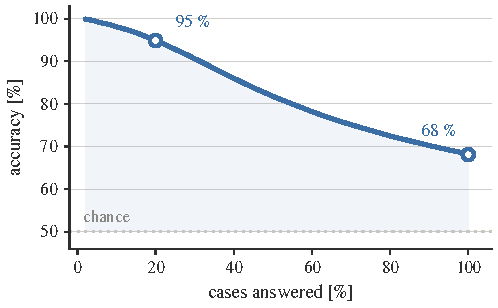
\includegraphics[width=0.948\columnwidth]{fig_coverage.pdf}
\caption{Accuracy against the share of cases answered, on the held-out
quarter, a case being one pair of routes. Moving left, the model answers
fewer cases, lowest confidence dropped first, and is right more often;
the dotted line is chance.}
\label{fig:coverage}
\end{figure}



% Cut for space 2026-09-07 (a claim about the reader rather than evidence;
% two readers flagged the paragraph as carrying none): That was not
% self-evident beforehand.
% Cut for space 2026-09-07 (the paragraph above has just given the delay
% rule's accuracy and the share of pairs it can decide): The delay rule is
% the instructive case, being accurate on the pairs it can decide and
% silent on the remaining 85.4\,\% of the archive, which is exactly the
% gap a learned model closes.

% Cut for space 2026-09-07 (a whole secondary point; the paper makes
% twelve such "this does not establish" moves and this is the least
% load-bearing of them, the ceiling of the task being a question the
% paper does not set out to answer. The journal version keeps it):
% That margin does not establish that 68.1\,\% is anywhere near the
% ceiling of this task. Part of the residual error falls on pairs in which
% the two routes are nearly indistinguishable on every recorded quantity,
% and part on decisions driven by information that no route-level dataset
% contains (e.g., slot swaps, crew legality, curfews or company routing
% policy). Neither share is separable from genuine model error without
% data that the network does not hold.

Where those 68.1\,\% sit is more informative than the pooled figure, and
Table~\ref{tab:strata} splits the quarter three ways. Accuracy climbs
steeply with the delay carried by the abandoned route, from 63.9\,\%
where there was none to 84.5\,\% between half an hour and an hour, where
the climb stops. That is what an economic reading predicts, since the
larger the delay, the clearer the incentive and the easier the decision
is to predict.
% Cut for space 2026-09-07 (the third block of the same table makes this
% reading two paragraphs later, with its evidence): The model is
% accordingly strong precisely where an airline is trading fuel against
% delay and the stake is large, and weak precisely where the two routes
% cost almost the same and the choice carries little consequence either
% way.

% Cut for space 2026-09-08 (the cost-inversion argument; the journal
% extension carries the same table and the full reading):
% One might expect the model to be most accurate when all cost indicators
% favour the move, but the third block of the table shows the opposite.
% When the newly filed route is not lower on any of the three direct costs
% (flight time, planned fuel, route charges), the model is right
% 79.9\,\% of the time; when it is lower on all three, only 53.9\,\%. On the 42.9\,\% of the first
% stratum where the route is strictly worse on every cost, accuracy
% reaches 86.3\,\%, so the model is strongest precisely where the costs
% offer no explanation for the move.
% Regulation exposure explains part of the gap: a regulation is present on
% 42.2\,\% of the first stratum against 33.7\,\% of the last. Those 8.5
% points of difference are not enough to account for 26.0 points of
% accuracy, but the direction is clear: the model contributes most where
% cost logic fails, which is where a system meant to complement cost
% models should contribute.
% CORRECTED 2026-09-06: the row was read as "worse on every recorded cost"
% (42.9% of it) and the contrast explained by a regulation "almost always"
% (42.2% against 33.7%). run_23_referee_checks.py.

\begin{table}[t]
\caption{Accuracy by stratum on the held-out quarter, with Wilson 95\,\%
intervals. The two blocks split the same 281\,720 pairs by regulation
exposure and by the delay attributed to the abandoned route.}
\label{tab:strata}
\centering\footnotesize
\begin{tabular}{lrr}
\toprule
stratum & pairs & accuracy [\%] \\
\midrule
\multicolumn{3}{l}{\emph{which route carried a regulation}} \\
\quad neither          & 178\,370 & 64.0 [63.8, 64.2] \\
\quad old route only   & 30\,953  & 88.0 [87.6, 88.3] \\
\quad both             & 67\,587  & 70.6 [70.2, 70.9] \\
\quad new route only   & 4\,810   & 58.6 [57.2, 60.0] \\
\midrule
\multicolumn{3}{l}{\emph{delay on the abandoned route}} \\
\quad none             & 205\,205 & 63.9 [63.7, 64.1] \\
\quad up to 15 min     & 19\,672  & 70.3 [69.7, 71.0] \\
\quad 15 to 30 min     & 18\,283  & 79.3 [78.7, 79.9] \\
\quad 30 to 60 min     & 21\,231  & 84.5 [84.0, 85.0] \\
\quad above 60 min     & 17\,329  & 83.5 [82.9, 84.0] \\
% Cut for space 2026-09-08 (cost-indicator stratum dropped with the
% cost-inversion argument; the journal extension carries the full table):
% \midrule
% \multicolumn{3}{l}{\emph{cost indicators favouring the new route}} \\
% \quad 0 of 3           & 90\,961  & 79.9 [79.7, 80.2] \\
% \quad 1 of 3           & 87\,471  & 70.0 [69.7, 70.3] \\
% \quad 2 of 3           & 78\,552  & 56.8 [56.5, 57.2] \\
% \quad 3 of 3           & 24\,736  & 53.9 [53.3, 54.5] \\
\bottomrule
\end{tabular}
\end{table}

A model that scores well on average but decays from month to month is not
deployable, and across April, May and June accuracy moves between
67.5\,\% and 69.0\,\%.
% Cut for space 2026-09-07 (a whole secondary point; the journal
% extension measures ageing directly, month by month over half a year,
% which is what the question actually needs):
% A replication fitted on 2025 alone, and without the stay-pair
% correction of Section~\ref{sec:changebias}, scores 67.3\,\% and
% 67.5\,\% on its own two test months, against the 68.9\,\% that the
% same uncorrected variant reaches on the main split.
% CORRECTED 2026-09-06: "the same recipe" was wrong; the model behind those
% two months is model_repl_nostay_seed42 ("stay_augmented": false), so the
% like-for-like comparator is 68.9%, not 68.1%.
% Cut for space (unverifiable from any exhibit in this paper, and the
% journal extension measures ageing directly over six months):
% Those five months span a schedule change, and accuracy does not step
% down across it.
% Cut for space (the journal extension measures model ageing directly):
% the 2025 replication was fitted to September and tested on November and
% December; March 2026 is the last month of the winter season and April
% the first of the summer one, when route availability, traffic and
% airline schedules change together; the best of the six months is the
% last one.
A quarter of evidence rules out rapid decay, but it does not establish
the retraining cadence a deployed system would need.

\subsection{Change bias}
\label{sec:changebias}
\label{sec:ablation-sec}

% Cut for space 2026-09-08 (the entire ablation table and its discussion;
% the journal extension reports every variant at full scale):
% Five design choices went into the model, and each was tested by
% retraining without it. Table~\ref{tab:ablation} reports the result, and
% one choice dominates the rest.
% [ablation table: indicators absolute -10.0, without stay-pair +3.7,
%  with monotone -0.2, without waypoint +0.03, vertical-only -2.0]
% The dominant choice is expressing the indicators relative to the other
% route: removing it costs nearly ten percentage points. The waypoint text
% is worth 1.4 percentage points at full scale (68.2 against 66.8), a
% real but secondary contributor. The weight w = 10 takes nearly all of
% the available correction at the smallest cost, and the tuning month
% selects it as well.

Section~\ref{sec:method} noted that most regulated revisions in the
archive move away from delay, so a model trained only on revisions
overweights delay as a negative signal and never sees the flights that
accepted a delay and kept their route. Stay pairs correct this by adding
such flights to both the training and the evaluation set.

The effect is clear on both populations. Trained on revisions alone, the
model scores 68.9\,\% on the revision pairs of the held-out quarter but
only 34.8\,\% on the 1\,093 stay pairs: whenever a flight stayed
despite a delay, the model predicts the wrong route. Adding stay pairs
at group weight~10, meaning each stay pair counts ten times as heavily as
one revision pair in the ranking loss, raises the stay-pair accuracy to
90.0\,\% and brings the revision accuracy to 68.1\,\%, a cost of
0.8~points.
Table~\ref{tab:strata} confirms that the adopted model also scores
88.0\,\% on flights that changed route after a regulation (the
\emph{old route only} stratum), so the correction does not trade one
population for the other.
% Cut for space 2026-09-08 (mirror-population argument replaced by a
% table cross-reference; the journal extension carries the full argument):
% The mirror population confirms that the correction works for the right
% reason. The adopted model scores 90.0\,\% on the 1\,093 stay pairs and
% 88.0\,\% on the 30\,953 escapes (flights that did change route after a
% regulation) of the same quarter. A rule using regulation status alone
% would be right on every stay pair and wrong on every escape, so it
% cannot produce both figures; the model must be reading the route and the
% flight around it, not just whether a regulation was present.

\subsection{Error analysis and feature attribution}

Errors concentrate where the model is already unsure. Among the quarter
of pairs whose two routes score furthest apart, only 5.6\,\% of all
errors fall, against the 25\,\% expected if error were independent of
confidence. In practical terms, most wrong predictions are cases the
model was nearly indifferent about, and a channel that abstains on those
cases avoids most of its mistakes.
% Cut for space 2026-09-07 (restates this paragraph's own opening
% sentence): Errors therefore concentrate at low confidence, which is what
% makes confidence filtering work.
% CORRECTED 2026-09-04: the 25 % reference applies to the quartile
% statistic alone; the near-tie share is a threshold
% (run_07_performance_analysis.py:367).
% Cut for space 2026-09-08 (the metric was opaque to readers without a
% concrete anchor): Most errors are near-ties: 27.7\,\% land within one
% fourth of the archive's median score gap.
% Cut for space 2026-09-07 (a whole secondary point, and the second
% single-case narrative in one section; Section V-D already follows a
% case from end to end. The journal version keeps it):
% The confident errors are nevertheless instructive, as one case from
% the held-out quarter shows: a flight re-filed off a route carrying 124
% minutes of attributed delay onto a route with none, saving fuel and
% time, and the model confidently scored the abandoned route higher. The
% flight-level context is identical within a pair by construction,
% and here every route-level quantity the model reads except the
% waypoint sequence favoured the move, so the preference came from the
% waypoint sequence, presumably a learned structural preference that
% overrode the rest. Confident errors are therefore not all of the
% hidden-information kind.
% Cut for space (the same gloss is given where the term is introduced, in
% Section IV-A: "decisions driven by information that no route-level dataset
% contains (e.g., slot swaps, crew legality, curfews or company routing
% policy)"): , meaning decisions driven by facts that appear in no
% route-level record, such as a slot swap or a curfew.
% Cut for space (the journal version develops it; a zero-context reader
% also read it as contradicting the proposal policy of Section IV-B):
% Opportunely, confident errors of this kind cost less than their share
% of the error rate suggests: the only route the channel could have
% offered is the cheaper one, the flight had just filed it, and a deployed
% channel, which unlike this simulation knows what is on file, would have
% said nothing at all.
The expensive errors are the opposite kind: the model confidently
proposes a route that the operator declines. A deployed channel has no
direct measure of that rate, because confident errors on stay pairs,
where the model wrongly advises leaving a route the airline kept, are the
closest available proxy, and that rate is the 10.0\,\% complement of the
90.0\,\% of Section~\ref{sec:changebias}.

A ranking model an operational user is asked to trust must be open to
interrogation, and Shapley attributions were therefore computed over
the held-out quarter~\cite{lundberg2017}.
Because the model decides on a comparison rather than on one route, what
Fig.~\ref{fig:shap} reports is the \emph{difference} between a feature's
attribution on the two routes of a pair, averaged in magnitude over the
quarter: both routes receive Shapley values for each feature, and the
plotted quantity is how much more the feature contributed to the
preferred route's score than to the other's. That is a ranking not of
what correlates with acceptance, but of what moves this particular
model's decisions.
% Cut for space: the game-theoretic reading, in which each feature is a
% player entering a room in random order and its attribution is the average
% change in the payout to the coalition already there.

\begin{figure}[t]
\centering
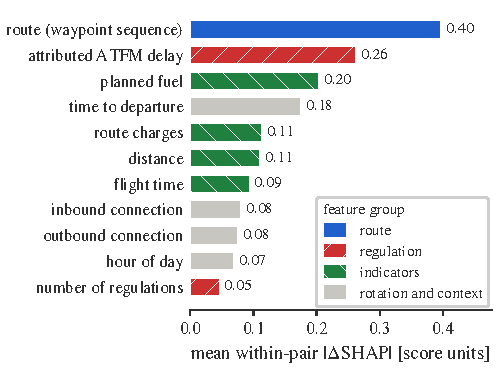
\includegraphics[width=0.948\columnwidth]{fig_shap.pdf}
\caption{What moves a decision: the mean absolute \emph{difference}
between a feature's Shapley value on the two routes of a pair, over
the held-out quarter, with the rotation and context groups of
Table~\ref{tab:features} drawn together. The waypoint sequence is the
largest single term, ahead of every \emph{individual} cost indicator,
though the four taken together sum to more; attributed ATFM delay
outweighs planned fuel. Rotation and context features are identical on
both routes, so their bars measure interaction rather than preference.}
\label{fig:shap}
\end{figure}

On that scale the waypoint sequence moves the score by 0.40, attributed
ATFM delay by 0.26 and planned fuel by 0.20, so route structure carries
information about the choice that the cost indicators do not.
% Cut for space (the figure and its caption already rank the terms):
% The waypoint sequence is the single largest term, ahead of every
% \emph{individual} cost indicator though the four together sum to more,
% which means that route structure carries information about the choice
% that the cost indicators do not. Attributed ATFM delay comes next,
% moving the score more than planned fuel does.
% CORRECTED 2026-09-04: the stated reason, the relative magnitude of the
% two quantities, cannot hold for a tree ensemble, which is invariant to
% the scale of a feature. The study does not establish why delay outranks
% fuel, so the claim is now confined to what was measured.
% Cut for space 2026-09-07 (a caution about an artefact of the exhibit
% rather than a finding, and the longest of the paper's remaining
% secondary points; the journal version keeps it in full):
% The rotation and context entries are a caution rather than a finding:
% What the figure ranks, in either case, is what moves this model's
% decisions and not what an operator values.
% time to departure appears fourth, with the inbound connection, the
% outbound connection and the departure hour below it. Three of those four
% are identical on both routes by construction, so what is measured for
% them is their interaction with the features that do differ; the outbound
% connection is the exception noted in Table~\ref{tab:features}, and does
% differ.

% Cut for space (the journal extension reports the occlusion study in
% full): descending to individual waypoints sharpens the picture, in that
% deleting a single identifier from a route and rescoring shifts the score
% by up to 2.5 points for the most influential one, and the affected
% waypoints cluster in a few places along the track rather than spreading
% evenly, which indicates that what the model has acquired is
% route-specific structure rather than a general preference for shorter
% routes.

The waypoint text ranks first by attribution, yet removing it and
retraining costs only 1.4 points of accuracy (68.2 against 66.8).
The two numbers answer different questions: attribution measures how much
the feature moves the score of the model that has it, while ablation
measures how much worse a model trained without it would be. Where
features are correlated, as route geometry and cost indicators plainly
are, the model trained without the waypoint text recovers part of the
lost information through the remaining features, so the ablation cost is
smaller than the attribution rank would suggest.

\subsection{What a channel would deliver, and the conditions for it}

% Cut for space 2026-09-07. The worked proposal followed one flight from
% end to end. It is the largest single block in Section V, the author's
% 2026-09-07 review asked for that section to be shorter and lighter, and
% the journal extension carries the same case in full with its distance,
% its median comparison and its levels. Everything it established is
% stated elsewhere: tau = 0.600 and the 79.2 %% in the paragraph on the
% channel's yield, the one-in-five proposal rate in the Conclusions, and
% the meaning of the validation in the deployment conditions below.
% RESTORE THIS FIRST if a page becomes available.
% One case from the held-out quarter shows what the channel is for, and
% every step below is a step the deployed system would take. A narrow-body
% was filed on a medium-haul sector, with no regulation attributed to
% either route. The system first takes the route then on file and the one alternative
% offered against it, computes their indicators as differences within
% the pair, and finds that the alternative burns 2\,016\,kg less planned fuel, close
% to a quarter of the trip fuel, at essentially the same distance and flight
% time. That margin is chosen because it is unambiguous, and it is far from
% typical: the median confirmed proposal saves 130\,kg.
% Cut for space 2026-09-07 (Section IV-A states the harmonisation rule
% this sentence restates): Both routes carry the same flight-level
% context, so nothing the model sees distinguishes them except where they
% go and what they cost.

% The model then scores each route, and the alternative comes out $+3.7$
% ahead on that same unitless scale: this is the pair whose two scores,
% $-2.82$ and $+0.90$, illustrated calibration in
% Section~\ref{sec:proposals}. That margin is not yet a decision: it passes
% through the calibrator fitted on the tuning month, which converts it into an
% acceptance probability, and that probability is compared with the threshold
% $\tau = 0.600$ fixed before the evaluation period began. This case clears it and the policy therefore proposes; had the margin
% been smaller the flight would have been left alone, which is what
% happens on roughly four flights in five.

% The operator's own later filing chose exactly that route. Keep in mind,
% however, that the airline was told nothing, so this is evidence not that a
% proposal would have been accepted, but that the model identified, before
% departure, a route the airline went on to prefer. That is the strongest
% validation available without running the channel, and the form on which
% every fuel figure here rests.

% Cut for space: Nothing about this flight is exotic: it carried no delay,
% it faced no regulation, and the saving came from a different track rather
% than from a shorter one. It is the ordinary case that a proposal channel
% exists to surface.


The question that remains is what a proposal channel built on this model
would deliver in practice. Three conditions stand between these results
and deployment. First, the delay attributed to a flight depends on which
regulations are active at the time the model scores it, and that picture
changes continuously as volumes open, close or shift their rates, so the
channel must score with the regulation state of the moment rather than
with a snapshot that may already be stale; the constraint is data
freshness, not computation. Secondly, a deployed channel would see every
flight, including the majority that never revise their plans, a
population on which the model was evaluated only through the 6\,672 stay
pairs of Section~\ref{sec:changebias}. Thirdly, acceptance itself is
never observed in this study; every figure rests on what the airline
filed next rather than on a response to an actual proposal.
% Cut for space 2026-09-07 (the last two conditions are stated again, with
% their evidence, in the Conclusions):
% so the model would be asked a question on which it was evaluated only
% through the stay pairs of Section~\ref{sec:changebias}; contentment with
% the filed plan is only one of the reasons a flight does not revise, and
% what the airline filed next is the strongest evidence available until
% proposals are actually made.

% Cut for space (the same point is made in Section II-B): Fortunately, a
% channel also generates exactly the data that would close this second gap,
% since every proposal answered is a new labelled observation of the very
% kind that the archive cannot supply; as those responses form a biased
% sample of the flights that the channel itself selected, the shadow-mode
% trial proposed as future work comes first.

At the operating point fixed in advance for 80\,\% precision
($\tau=0.600$, delivering 79.2\,\%), the simulated channel surfaces
56\,162 proposals over the held-out quarter. Those proposals carry
20.1\,kt of planned-fuel savings, counted only where the airline's own
later filing chose the route proposed to it, or 63.5\,kt of CO$_2$ at
3.16\,kg per kilogramme of fuel. Annualised, that is between 222 and
254\,kt of CO$_2$. The two bounds differ because the held-out quarter
falls in spring and summer, when traffic is above the annual average:
multiplying the quarter by four gives 254\,kt, while applying the
per-flight saving rate to twelve months of eligible traffic gives
222\,kt.
The channel figures are computed on
flights that revised their plans, and planned fuel is the dispatcher's
estimate filed before departure, not the fuel actually burned, so
they should be read as what a channel could have surfaced earlier rather
than as a traffic-wide counterfactual. The full channel analysis is the subject of a journal extension of
this work.

Figure~\ref{fig:example} follows one of these proposals through the
scoring pipeline. A narrow-body was filed on a medium-haul route with no
regulation; the alternative saves 2\,016\,kg of planned fuel at
essentially the same flight time but 227\,EUR more in route charges. The
model scores the alternative 3.7 above the filed route, the calibrator
maps that gap to a 99\,\% acceptance probability, well above
$\tau = 0.600$, and the channel proposes. The airline's later filing
chose exactly that route. The margin is far from typical: the median
confirmed proposal saves 130\,kg, but this case shows every step of the
pipeline in one place.

\begin{figure}[t]
\centering
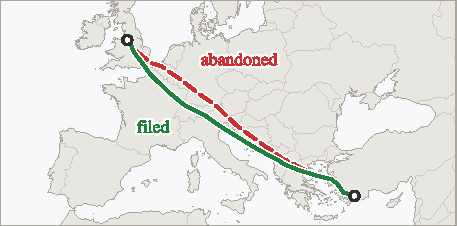
\includegraphics[width=0.88\columnwidth]{fig_example_map.pdf}\\[2mm]
\footnotesize
\setlength{\tabcolsep}{5pt}
\begin{tabular}{@{}lrr@{}}
\toprule
 & \textit{abandoned} & \textit{filed} \\
\midrule
planned fuel [kg]       & 10\,485 & 8\,469 \\
flight time [min]       & 259     & 258 \\
route charges [EUR]     & 2\,269  & 2\,496 \\
\midrule
model score             & $-2.82$ & $+0.90$ \\
\bottomrule
\end{tabular}\\[2mm]
gap $= 3.7 \;\longrightarrow\; P = 0.99 \;>\; \tau = 0.600 \;\longrightarrow$ proposed
\caption{A worked example from the held-out quarter. The route
initially on file (dashed red) and the fuel-saving alternative (solid
green) are shown on an anonymised city pair. The alternative saves
2\,016\,kg of planned fuel at 227\,EUR more in route charges and
the same flight time. The calibrated acceptance probability exceeds the
threshold; the airline's own later filing chose the proposed route.}
\label{fig:example}
\end{figure}

% =====================================================================
\section{Conclusions} \label{sec:conclusions}

Airline route acceptance is learnable from flight-plan revisions at network
scale. A model fitted on
1\,134\,000 revisions identifies the chosen route in 68.1\,\% of held-out
cases, 13.1 points above the best rule built on any one indicator, and its
confidence is informative enough to choose where to operate rather than
settle for a single accuracy figure: on the fifth of decisions it is most
confident about, it is right 94.9\,\% of the time. The model weighs route
structure more heavily than any individual cost indicator, though removing
the waypoint text costs only 1.4 points, so what it contributes is real
but secondary. It is nonetheless information that a formulation based on
costs alone cannot represent.
% Cut for space 2026-09-08 (the cost-inversion conclusion, dropped with
% the argument it rested on):
% Secondly, that margin is widest exactly where cost logic fails, 79.9\,\%
% where no cost indicator favours the route the airline moved to against
% 53.9\,\% where all three do.

The number that characterises this system is not 68.1\,\% but the curve of
Fig.~\ref{fig:coverage}, because a channel chooses where on that curve to
sit, and because ranking a pair correctly and proposing correctly are
different quantities of which the second is the operational one: at
the threshold used here, the channel proposes on about a fifth of the
flights whose two routes differ in planned fuel at all, and 79.2\,\% of
those proposals match what the airline went on to file. Accordingly, a first deployment would sit at low coverage on
Fig.~\ref{fig:coverage}, answering only the cases it is most confident
about, and would widen that coverage only as acceptance is observed.

Two bounds remain. The first is the population the second deployment
condition names: the data on flights that stayed is small,
6\,672 pairs in all and 1\,093 in the test months, and each stay pair
joins two different flights rather than two routes filed for the same
flight, so a model could learn to recognise how the pair was built rather
than the preference it encodes. The stay-pair accuracy of
90.0\,\% in Section~\ref{sec:changebias} shows that the model is not
simply reading regulation status, but it cannot rule out subtler
artefacts of the construction.

The second lies in how a route is represented. The model reads a route as
the ordered sequence of waypoint names along it, so what it holds about
route structure is a vocabulary, not a geometry. Those names are
European: a waypoint such as KONAN or MAROT exists only in this
region's airspace, so little of the 1.4 points the waypoint text is
worth would survive a move to another continent. They are also revised
periodically, so a piece of airspace can return under a name the model
has never seen.

We tested the obvious alternative: a Transformer encoder was trained on
geometric route descriptors (shape alone, no names) and its embeddings
were fed as additional features into CatBoost. The hybrid scored below
the model that uses the text tokens directly, and a linear classifier on
the embedding differences separated preferred from abandoned routes at
little better than chance, which points at the geometric input rather
than the training objective as the limitation.
% Cut for space 2026-09-07: Those trials predate a repair to this archive,
% so only their ordering is claimed. (Recorded in the journal version and
% in AUTHOR_REVIEW_2026-09-07.md; no accuracy from them is quoted here.)
% Absolute numbers from research_ideas.md: CatBoost+BoW 74.9%,
% CatBoost+embeddings(128-dim) 72.7%, linear probe on embeddings 57.4%,
% route-only contrastive encoder probe ~54%. Not quoted in paper because
% they predate the 2026-09-01 archive repair.
A name-independent representation of route shape is nonetheless what
would make this model portable, and remains worth pursuing.

A related limitation is that fuel appears in the feature set as
kilograms of planned fuel, not as a cost. A kilogram of jet fuel in 2025
and a kilogram in 2035 will not carry the same price, so the relative
weight an airline places on fuel against, say, route charges in euros
will shift as fuel costs change. Recasting fuel as a monetary cost, or
normalising all indicators to a common unit, would make the model's
trade-offs more stable across years.

Future work should therefore begin with a balanced stay dataset in which
regulation status is independent of the label, which requires data that
is not currently assembled rather than data that does not exist. A
shadow-mode trial logging the real responses of operators would close the
remaining gap.

\section*{Disclaimer}
The views expressed are those of the authors and do not necessarily reflect
the official position of EUROCONTROL or of its Member States. This paper
reports research and does not commit to any operational service.

\balance
{\footnotesize
\bibliographystyle{IEEEtran}
\bibliography{refs}
}

\end{document}
